% Number 1010
% NAPM Calculus Algebra Units 
% NAPM vs. CAPM, modeling and graphing
% JG

% Watermark
\AddToShipoutPicture*{\BackgroundPic}

\addtocounter {ProbNum} {1}

%\begin{floatingfigure}[r]{.44\textwidth}
%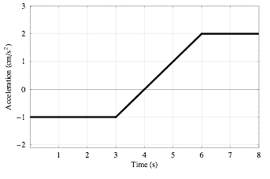
\includegraphics[scale=.95]{/Users/jgates/desktop/latex/pics/agraph1}
%\end{floatingfigure}
 
{\bf \Large{\arabic{ProbNum}}} An object starts from rest at $x=0$ at time $t=0$. Five seconds later, the object is at $x=40~m$ and is velocity is ${+11~\tfrac{m}{s}}$. \bigskip

Was the object's acceleration constant or non-constant during this interval? Explain/give evidence to support your reasoning.
\paragraph{}
\noindent
\vfill

Sketch the velocity graph implied by these data. Is the graph linear or curved? If it is curved, is it concave up or down?
\vfill

%\begin{center}
%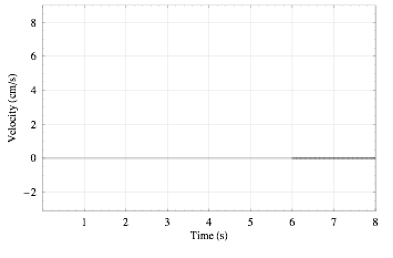
\includegraphics[scale=.7]{/Users/jgates/desktop/latex/pics/vgraph8}
%\end{center}



\newpage